\begin{frame}{Ziele}{im userspace}
 \begin{itemize}
  \item \cod{open}, \cod{read}/\cod{write}, \cod{close}
  \item zwei {\em flavours}
  \begin{itemize}
   \item low-level I/O
   \item I/O on streams
  \end{itemize}
 \end{itemize}
\end{frame}

\begin{frame}{Alles ist ein File}{etwas genauer}
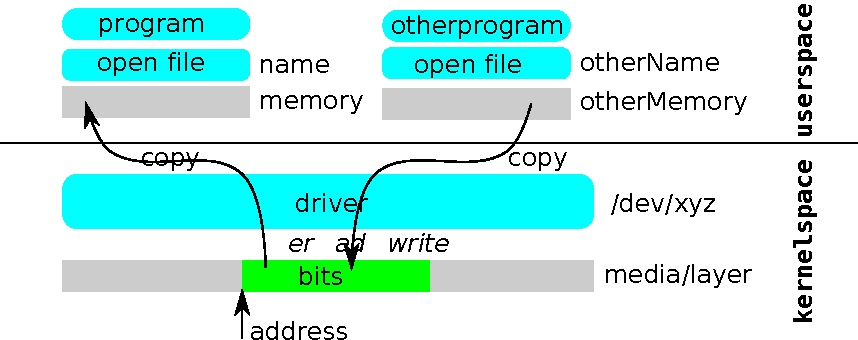
\includegraphics[width=0.875\textwidth]{driver-file.pdf}
%\includesvg{driver-file}
\end{frame}


\begin{frame}{Beispiele}
 \begin{itemize}
  \item \cod{low-level-io.c}
  \item \cod{io-level-on-streams.c}
 \end{itemize}
\end{frame}

\subsection{Aufgaben}
\begin{frame}{Aufgaben}
\begin{itemize}
 \item \cod{low-level-io.c}/\cod{io-level-on-streams.c} für \host und \targetS
\end{itemize}
\end{frame}
